\chapter{Escopo}
\label{escopo}

\section{Metodologia de elucidação do escopo e do produto}

\par \textit{Lean Inception} é o nome dado ao método colaborativo para alinhar um grupo de pessoas sobre o MVP (produto mínimo viável) que será desenvolvido. É uma sequência de atividades para alinhar e definir objetivos, estratégias e o escopo do produto.\cite{caroli2014lean} 
\par O produto mínimo viável, em Inglês\textit{  Minimum Viable Product} (MVP), é a versão mais simples de um produto que pode ser disponibilizada para o negócio. O MVP determina quais são as funcionalidades mais essenciais para que se tenha o mínimo de produto funcional que possa agregar valor para o negócio (produto mínimo) e que possa ser efetivamente utilizado e validado pelo usuário final (produto viável). \cite{moogk2012minimum}
\par O nome\textit{ Inception }vem do RUP (\textit{Rational Unified Process}). \textit{Inception} é a primeira de quatro fases do RUP: \textit{Inception, Elaboration, Construction e Transition.} Na fase de \textit{Inception} é realizada a análise sobre os objetivos, a arquitetura e o planejamento do projeto. Isso acontece por meio de entrevistas com os \textit{stakeholders}, reuniões de alinhamento e dinâmicas de equipe. As informações obtidas nessas atividades são convertidas em requisitos descritos no formato de casos de uso. \cite{caroli2014lean} 
\par Apesar de a metodologia RUP ter sido adotada pela equipe, optou-se por não utilizar  casos de uso para delimitar as funcionalidades do produto, pois eles caíram em desuso, e os métodos ágeis adotaram o formato de histórias do usuário, que são mais focadas nos usuários do produto e entregam mais fidelidade sobre as necessidades destes. Assim, podemos definir nosso desenvolvimento do produto como \textit{user centered development}. Portanto, seguindo a nova metodologia adaptada, atividades sobre os usuários e suas jornadas são feitas (influência de \textit{design thinking} e \textit{user-centric design}); muitas histórias dos usuários são escritas, estimadas, arquitetadas e colocadas em um plano: o plano de \textit{release} do produto. 
Para elucidar e definir os requisitos, as técnicas utilizadas pela equipe foram as seguintes: 
\begin{itemize}

\item Escrita da visão de produto dinamicamente 
\item Desenvolvimento de um diagrama de causa e efeito 
\item Elaboração da estrutura analítica do projeto 
\item Método \textit{Rich Picture} 
\item Definição dos objetivos gerais e específicos
\item Definição dos requisitos 
\item É /não é, faz/não faz

\end{itemize}
\par Nos tópicos a seguir, pode-se verificar em detalhes como cada artefato foi elaborado, bem como os resultados obtidos a partir de cada artefato gerado pela equipe.
\section{Escrita da visão do produto dinamicamente}
\par Antes de iniciar a construção do produto, é importante que seja estabelecida uma visão compartilhada junto à equipe e aos demais envolvidos. Esse artefato, portanto, ajuda a manter o foco e a clareza quanto aos objetivos do produto e proporciona a horizontalidade e a distribuição de conhecimentos em relação esse produto. Uma das maneiras encontradas pela equipe para realizar essa atividade foi a elaboração de uma dinâmica de escrita da visão do produto de forma dinâmica, onde após toda a equipe reunida, realizou-se uma dinâmica de escrita coletiva de pontos importantes para a realização do produto. Após a dinâmica, foi gerado um artefato resultante que foi disponibilizado para a equipe e os \textit{stakeholders}. 

\begin{figure}[H]
\centering
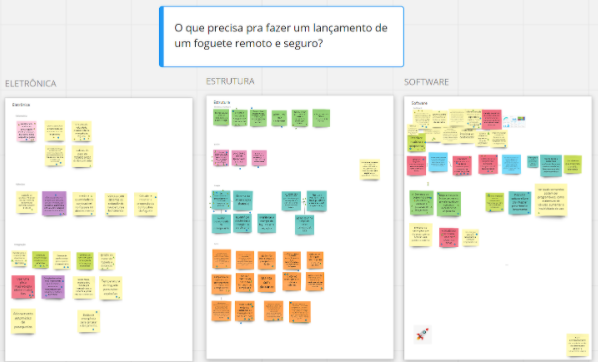
\includegraphics[scale=0.8]{figuras/miro.png}  
\caption{Ideias iniciais para solucionar o problema.}
\footnotesize Pode-se acessar em: \url{https://miro.com/app/board/o9J_kmVCAxA=/ }
\label{fig:miro }
\end{figure}

\section{Objetivos Gerais}

\par O objetivo geral do projeto é desenvolver uma tecnologia que proporciona de maneira segura o controle a longa distância do lançamento de foguetes de pequeno porte e a transmissão dos dados de voo para a central de comando (\textit{Ground Station}), ou seja, uma estação de controle de solo onde é possível controlar o abastecimento e o lançamento do foguete e receber os dados coletados durante o voo por uso da telemetria, contendo um interfaceamento intuitivo e versátil para o usuário.

\section{Objetivos Específicos}

\subsection{Eletrônica}

\par O subgrupo de eletrônica tem como objetivo  desenvolver a solução de sistema embarcado que será utilizado no projeto o que inclui: a) telemetria, que consiste no modo de transmissão de dados e sinais de controle a longas distâncias; b) sensoriamento, que consiste na captação dos estímulos físicos e a emissão de  sinais que possam ser convertidos novamente nos dados relevantes para análise do voo do foguete; c) hardware principal, que permite interfaceamento com o usuário.

\par Primeiramente serão levantados os requisitos, em conjunto com as áreas de software e energia, para melhor definição da solução e dos componentes. Em seguida, com a definição dos componentes, será feita uma bateria de testes dos sensores e periféricos com microcontroladores e microprocessadores,Umas das técnicas mais populares para documentar ideias de maneira rápida é o brainstorm. No entanto, essa técnica exige muito esforço para ser aplicada em grupo devido a dificuldade de organização das ideias e do gerenciamento de conflitos.
O brainwriting é a aplicação da técnica do brainstorm de maneira silenciosa, proposto para substituir o brainstorm em grupos. 
“Brainwriting é a geração silenciosa e escrita de ideias por um grupo de pessoas”
Existem 6 maneiras distintas de se fazer um brainwriting,
Nominal Group Technique (NGT)
Collective Notebook (CNB)
Brainwriting Pool
Pin Cards
Battelle-Bildmappen-Brainwiiting (BBB)

Para execução do brainwriting no nosso contexto, foram feitas algumas adaptações a partir do entendimento e aplicação de cada uma das técnicas.
Foi utilizada uma combinação das técnicas “Brainwriting Pool” e  “Nominal Group Technique (NGT)”, resultando na seguinte definição:
O organizador deve identificar um tema central da sessão, um problema. 
Cada participante vai usar seu espaço no MIRO para fazer um brainstorm silencioso durante 5 minutos cronometrados.
Após os primeiros 5 minutos os participantes vão usar o espaço do colega do lado pra fazer suas próprias anotações por mais 5 minutos (pode se repetir). 
Após a segunda ou terceira interação (dependendo do organizador) cada participante volta para seu espaço e lê suas ideias para o grupo, nessa etapa os integrantes podem fazer perguntas e comentários para ajudar a entender melhor a ideia em questão.
Após todos integrantes terem lido e entendido o que foi feito, todas idéias serão agrupadas de acordo com sua similaridade ou proximidade.
Cada participante receberá 1 estrela, 3 triângulos e 5 bolas. Os elementos valem: Estrela - 5 pontos, triângulo 3 pontos, bola 1 ponto.
Critério de desempate: O critério de desempate é a quantidade de elementos com pontuação maior
Os integrantes terão 5 minutos para distribuir seus pontos entre as ideias selecionadas na etapa anterior.
Ao fim da dinâmica é feita a contagem dos pontos e eleição das ideias que serão aproveitadas pelo grupo em ordem de prioridade.


Utilizando essa metodologia, conseguimos estabelecer uma visão compartilhada junto à equipe e aos demais envolvidos sobre o produto que seria desenvolvido. O artefato gerado ajuda a manter o foco e a clareza quanto aos objetivos do produto e proporciona a horizontalidade e a distribuição de conhecimentos em relação ao mesmo.
 para que assim haja a implementação do conjunto que compõe o sistema como um todo. 
\par Por fim, os ajustes finos de calibração e integração com software serão priorizados, para que seja atingida uma melhor experiência por parte do usuário.

\subsection{Energia}
\par O subgrupo de energia teve como objetivo realizar o dimensionamento elétrico do sistema como um todo, para escolher as características de um banco de baterias que suporte a alimentação dos dispositivos em um intervalo de tempo desejado. Foi preciso levar em conta que o sistema é projetado para funcionar em locais remotos e, por isso, não será possível ligá-lo à rede elétrica.
\par Também será projetado um carregador móvel para que, após o lançamento, quando necessário, seja possível conectar o sistema à rede elétrica e assim carregar a bateria.

\subsection{Software}
\par Para garantir a eficiência no uso do equipamento, a equipe deverá implementar uma interface gráfica intuitiva e adaptativa que seja capaz de receber os dados de leitura realizados pelo hardware e, após uma análise, efetuar a estruturação dos dados. Além disso, deverá garantir que o controle do abastecimento, a ignição e a abertura do paraquedas do foguete aconteçam de forma remota por meio do envio de comandos executados pelo operador do equipamento.  
\par Também será realizada a captação de informações a respeito das condições climáticas, do estado de saúde do equipamento e das informações relacionadas ao lançamento e ao voo do foguete em tempo de execução. A equipe deverá também realizar a análise quantitativa dos dados obtidos e disponibilizar graficamente os resultados por meio do sistema. 

\subsection{Estrutura}
\par O subgrupo de estrutura ficou responsável pelo desenvolvimento físico da estação de controle e de três dispositivos periféricos, responsáveis pela atuação física da abertura e do fechamento de válvulas do sistema de alimentação do foguete.
\par Quanto à estrutura da estação de controle, será desenvolvido um \textit{case} capaz de comportar um sistema de hardware complexo, com componentes eletrônicos embarcados por um software de alto nível. É esperado que o sistema seja usado em locais remotos, com presença de elementos ambientais adversos, como poeira ou mesmo umidade. Essa estrutura deve ser ainda leve e facilmente transportável, o que influencia na escolha dos materiais de que será feita. Por fim, a estrutura da estação será dimensionada para possuir uma região de armazenamento para os componentes ignitores, além de garantir a proteção dos componentes internos contra eventuais cargas externas.
\par Das estruturas periféricas, a estrutura se encarregará, junto da eletrônica, do desenvolvimento de um sistema que faça a abertura física das válvulas do sistema de alimentação de forma remota. Nesse sentido, serão desenhadas estruturas que conectam as válvulas utilizadas nesse sistema com um sistema eletromecânico que consiga receber o sinal da estação e aplicar o torque necessário para abertura ou fechamento dessas válvulas.

\section{Requisitos Gerais}
\par O \textit{Rocket Guide Station} (RGS) será um equipamento criado com a finalidade de tornar mais fácil e seguro o lançamento de foguetes de propulsão híbrida, levando em consideração os requisitos gerais a seguir:

\begin{table}[H]

\begin{tabular}{ | m{2cm} | m{12cm}|} 
 \hline
 \textbf {Requisito} & \begin{center}\textbf{Descrição} 
 \end{center}\\ 
 \hline
 RGS01 & Realizar o abastecimento e o lançamento de foguetes de propulsão híbrida de pequeno porte de forma remota e segura. \\ 
 \hline
 RGS02 & Obter informações relativas ao voo do foguete em tempo real.	 \\ 
 \hline
\end{tabular}
\caption{Requisito Gerais}
\label{Requisito Gerais}
\end{table}

\section{Requisitos Específicos}
\subsection{Estrutura}


\begin{table}[H]
\begin{tabular}{ | m{2cm} | m{12cm}| } 
 \hline
 \textbf{Requisito} & \begin{center}\textbf{Descrição}
   
 \end{center} \\ 
 \hline
 RFEST01 & Ser de uso intuitivo para o usuário.\\
 & \\
\hline
 RFEST02 & Estrutura física compacta e portátil, que dê suporte aos componentes internos da estação. \\
 \hline
 RFEST03 & Material leve e resistente, capaz de proteger os componentes internos da estação de eventuais impactos e intempéries provenientes do ambiente e de seu deslocamento. \\
  \hline
RFEST04 & Possuir um espaço na estrutura para o armazenamento do sistema de ignição. \\
\hline
RFEST05 & Ter um sistema de transmissão de torque do atuador para a válvula-esfera do sistema de abastecimento. \\
\hline
RFEST06 & Proteger o sistema eletrônico e não gerar interferência neste.  \\
\hline
RFEST07 & Estrutura interna acessível e de fácil manutenção. \\
\hline
RFEST08 & Sistema de abastecimento baseado nos componentes definidos pelo cliente. \\
\hline
\end{tabular}
\label{Requisitos de Estrutura}
\caption{Requisitos de Estrutura}
\end{table}

\subsection{Software}

\begin{table}[H]
\begin{tabular}{ | m{2cm} | m{12cm}| } 
 \hline
 \textbf{Requisito } & \begin{center} \textbf{Descrição}\end{center}\\
 \hline
 RFSW01 & O sistema deve permitir interação do usuário com a interface.\\
 \hline
 RFSW02 & O sistema deve permitir ao usuário visualizar o índice de sucesso com base de modelos estocásticos do voo em tempo de execução. \\
 \hline
 RFSW03 & O sistema deve exibir dados relevantes para a análise do operador. \\
 \hline
 RFSW04 & O sistema deve armazenar informações sobre o lançamento e voo de foguetes de forma indexada. \\
 \hline
 RFSW05 & O sistema deve ser capaz de enviar sinais a periféricos. \\
 \hline
 RFSW06 & O sistema deve ser capaz de interpretar os dados recebidos dos periféricos. \\
 \hline
\end{tabular}
\label{Requisitos de Software}
\caption{Requisitos de Software}
\end{table}


\subsection{Eletrônica}

\begin{table}[H]
\centering
\begin{tabular}{| m{2cm} | m{12cm}| } 
 \hline
 \textbf{Requisito} & \begin{center}\textbf{Descrição}\end{center} \\ 
 \hline
 RFEL01 & O sistema deve realizar o controle de toda parte sensorial\\
 &acoplada aos microcontroladores e microprocessador.\\
 \hline
 RFEL02 & O sistema deve ser capaz de monitorar o peso do foguete antes do lançamento.\\ 
 \hline
 RFEL03 & O sistema deve mandar um sinal para o aquecimento da resistência da ignição do foguete.\\ 
 \hline
 RFEL04 & O sistema deve fazer o uso de telemetria para o colhimento dos dados do foguete e seu controle.\\ 
 \hline
 RFEL05 & A RGS deve comunicar-se numa distância mínima de 1.5Km.\\ 
 \hline
 RFEL06 & O sistema deverá funcionar independentemente do acesso à internet.\\ 
 \hline
\ RFEL07 & A comunicação entre o foguete e o controle do usuário deverá ser feita sem fios.\\ 
 \hline
 RFEL08 & Os controles do acionamento das válvulas, acionamento da ignição, aferição dos combustíveis e do peso, visualização dos dados de GPS altitude deverão estar integrados na interface do usuário. \\ 
 \hline
 RFEL09 &  O sistema deverá ter um \textit{display} para mostrar os dados de telemetria/monitoramento (Hardware +  Software).\\ 
 \hline
 RFEL10 &  O sistema deverá ter periféricos para interação com o usuário (botões ou teclado) (Hardware + Software).\\ 
\hline

\end{tabular}
\label{Requisitos de Eletrônica}
\caption{Requisitos de Eletrônica}
\end{table}


\subsection{Energia}

\begin{table}[H]
\centering
\begin{tabular}{ | m{2cm} | m{12cm}|} 
 \hline
 \textbf{Requisito} & \begin{center} \textbf{Descrição }\end{center}\\ 
 \hline
 RFEN01 & Sistema elétrico portátil que engloba o armazenamento de  energia e a alimentação do sistema  com dispositivos leves e compactos.\\
 \hline
 RFEN02 &  Autonomia energética para no mínimo 2 horas de operação e no máximo 3 horas (intervalo de tempo que leva em média para o lançamento do foguete). \\ 
 \hline
 RFEN03 & Sistema elétrico capaz de alimentar os dispositivos de ignição. \\
 \hline
 RFEN04 & Carregador móvel de bateria que utilizará a rede elétrica.\\

 \hline
\end{tabular}
\label{Requisitos de Energia}
\caption{Requisitos de Energia}
\end{table}


\subsection{Requisitos de Usabilidade }

\begin{table}[H]
\centering
\begin{tabular}{ | m{2cm} | m{12cm}| } 
 \hline
 \textbf{Requisito} & \begin{center} \textbf{Descrição} \end{center}\\ 
 \hline
 RUSW01  & A interação do usuário com a interface do produto deverá ser intuitiva.\\
 \hline
 RUSW02 & A interface deverá possuir prevenção e notificação de erros, caso o \\& preenchimento de dados for incorreto. \\ 
 \hline
 RUSW03 & O produto deve ser suficiente energeticamente durante o voo.\\ 
 \hline
 RUSW04 & As rotinas manuais de lançamento deverão ser, em sua maioria,  automatizadas.\\ 
 \hline
 RUSW05 & A estrutura deverá comportar os componentes eletrônicos da própria estação \\& e possuir um espaço sobressalente. \\ 
 \hline
 RUSW06 & Os módulos do sistema deverão comunicar-se por meio de rádio frequência.\\ 
 \hline
 
\end{tabular}
\label{Requisitos de Usabilidade}
\caption{Requisitos de Usabilidade}
\end{table}

\section{Lista É/Não É}
\par A dinâmica de É/Não É é uma atividade que ajuda a identificar o escopo, as limitações do produto e os aspectos que devem ser realmente considerados na hora do desenvolvimento. Trata-se de uma matriz onde, por meio de uma discussão de equipe, definem-se as características, e também aquilo que não serão características, do produto. O quadrante “É”, deve ser preenchido com tudo aquilo que o produto que será desenvolvido é, e o quadrante “Não é” com tudo aquilo que o produto não deve ser.

\begin{center}
\begin{table}[H]

\begin{tabular}{ | m{7cm} | m{7cm}| } 
 \hline
\begin{center}\textbf{É }\end{center} & \begin{center} \textbf{NÃO É}\end{center}   \\ 
 \hline
É capaz de receber e mandar dados de controle com o foguete e sua base. & Não é à prova d’água. \\ 
 \hline
 É capaz de mandar sinais de controle para válvulas do abastecimento e para ignição do foguete. & Não é capaz de parar o lançamento após a ignição. \\ 
 \hline
É capaz de colher dados de sensores no foguete e enviar para a visualização do usuário. & Não é capaz de comunicar-se a distâncias maiores que 2 km. \\ 
 \hline
É capaz de mostrar os dados por meio de uma tela. & Não é capaz de comunicar-se com a internet.\\ 
 \hline
 É capaz de receber comandos do usuário por meio de um teclado. & Não é um computador pessoal (uso geral). \\
 \hline
 É capaz de comunicar-se de forma sem fio entre os microcontroladores. & Não é capaz de desabastecer o foguete \\
 \hline
 É capaz de armazenar os dados dos sensores do foguete em uma memória externa. & Não é um sistema de lançamento autônomo. \\
 \hline
 É capaz de coletar GPS, velocidade e apogeu do foguete. & Não é capaz de coletar a pressão interna e temperatura dentro do foguete e dados sobre a qualidade do combustível. \\
 \hline
 É um sistema autônomo e móvel com uso de bateria. & Não é conectado de forma fixa à rede elétrica. \\
 \hline
 É carregado periodicamente conforme a necessidade. & Não é totalmente independente da rede elétrica. \\
 \hline
É base de comando. & Não é uma base de lançamento. \\
\hline
É estrutura comportadora de um hardware embarcado. & Não é um foguete experimental. \\
\hline
É um sistema independente do tanque de combustível. & Não é um tanque de combustível. \\
\hline
Tem ignição eletromecânica. & Não é uma mala comum de viagem. \\
\hline
\end{tabular}
\label{Lista de É/Não É}
\caption{Lista de É/Não É}
\end{table}
\end{center}

